\section{White Rabbit} \label{sec:wr}

\acrfull{wr} hace referencia tanto al protocolo diseñado como mejora de 
\gls{ptp}v2 como al proyecto internacional que se encarga de su desarrollo y 
mantenimiento. Inicialmente parte como una tecnología desarrollada por el 
\gls{cern} para actualizar el sistema de sincronización y envío de datos de 
control para su complejo de aceleradores de partículas. Gracias a el espíritu 
abierto con el que se desarrolló la tecnología (y a su prometedor rendimiento) 
fueron sumándose otras instituciones al desarrollo, tanto desde el ámbito 
académico, donde cabe destacar el Centro de Investigación de Iones Pesados 
(\textit{Gesellschaft für Schwerionenforschung}, GSI en alemán) en Alemania o 
la propia Universidad de Granada; como desde el empresarial, donde se está 
intentando expandir la tecnología al ámbito industrial. Ejemplos de ello son la 
empresa Seven Solutions (\text{spin-off} de la UGR) en Granada, o CreoTECH en 
Polonia. 

Aunque el empuje en el ámbito de la ciencia es mucho más 
evidente gracias a la inclusión de \textit{WR} en instalaciones para 
aceleradores de partículas, institutos metrológicos o en sistemas de 
adquisición ditribuida como el caso del proyecto Square Kilometre Array (SKA) 
que se está contruyendo en Sudáfrica y que una vez concluido será el 
instrumento de observación astronómica más sensible jamás construido por la 
humanidad. En el caso de la empresa privada, \gls{wr} se ve todavía como una 
tecnología muy prometedora para diversas áreas como Smart Grid, 
Geo-posicionamiento o para las telecomunicaciones, que aún necesita madurar. 
Esto está a punto de cambiar gracias a su inclusión en la próxima revisión del 
estándar \gls{ptp} bajo un nuevo perfil de alta precisión.

Los objetivos de desarrollo iniciales estaban enfocados al entorno de los 
aceleradores de partículas, priorizando una sincronización de calidad junto a 
un sistema que fuese determinista y fácil de mantener:

\begin{itemize}
	\item Lograr para una red de miles de nodos, conectados por enlaces de 
	fibra óptica de hasta 10 km, una diferencia menor del nanosegundo entre dos 
	nodos cualesquiera de la red, es decir, una exactitud de sincronización 
	\textbf{sub-nanosegundo}. Además, se requiere una precisión en el orden del 
	picosegundo.
	
	\item Permitir que el enlace utilizado para los paquetes del protocolo 
	\gls{wr} se pueda \textbf{compartir para} el envío de \textbf{datos de 
	propósito general}, 
	reduciéndo así costes en el despliegue de las infraestructuras.
	
	\item Realizar un desarrollo \textbf{simple y escalable} que no necesite de 
	sofisticados procedimientos de configuración o calibración.
	
	\item Establecer un envío \textbf{determinista} para los paquetes 
	prioritarios, con 
	retardos que no superen ciertos valores umbrales. Esto es especialmente 
	importante en sistemas de control donde la respuesta a un evento no puede 
	exceder un tiempo límite en su envío.
	
	\item Proveer un \textbf{diseño} de referencia \textbf{abierto} a la 
	comunidad 
	(tanto \textit{hardware} como \textit{software}) para fomentar el 
	desarrollo por parte de esta, y evitar las ligaduras con fabricantes.
\end{itemize}

En la actualidad se puede afirmar que en su mayor parte se han cumplido dichos 
objetivos. El requisito principal de rendimiento es algo que se ha conseguido 
en su mayor parte aunque hace falta aportar datos acerca del comportamiento del 
protocolo en redes realmente grandes con un gran número de nodos. La tendencia 
actual en cuanto a rendimiento se centra en la mejora de la exactitud alcanzada 
en escenarios no tan típicos, como enlaces de larga distancia o escenarios con 
cambios en las condiciones de operación. También se investiga como reducir el 
ruido producido por los componentes del sistema de sincronización para lograr 
una precisión en el orden del femtosegundo. El envío determinista es algo que 
no siempre se logra, ya que se puede producir la pérdida de algún paquete de 
alta prioridad en casos de congestión del enlace. Las herramientas de gestión y 
mantenimiento es otro punto al que todavía le queda trabajo por delante y al 
que se está prestando bastante atención dado que son algo crucial si se 
pretende extender el uso del protocolo más allá del ámbito científico.

El protocolo \gls{wr} fue diseñado como una extensión del protocolo IEEE 
1588-2008 (\gls{ptp}v2) al que se añadieron varias mejoras como un modelo de 
enlace más preciso, técnicas de calibración automática o sintonización de los 
relojes mediante el envío de la frecuencia maestra codificada en los paquetes 
transmitidos.

\subsection{Arquitectura de red}

Dado que WR parte del diseño del protocolo PTP, la estructura de la red es 
similar a la explicada en las secciones anteriores. La figura 
\ref{fig:wrtopology} muestra una red de tipo jerárquica donde se sitúa en la 
raíz el nodo maestro de toda la red (equivalente al Grand Master de PTP) y que 
suele enlazarse a una fuente de reloj muy estable. Opcionalmente pueden existir 
otros nodos que se sitúen en este nivel por temas de redundancia. Los 
siguientes niveles son equivalentes a los BC vistos en PTP, y por último se 
sitúan los equipos que actúan como nodo esclavo que serían equivalentes a los 
OC.

\begin{figure}
	\centering
	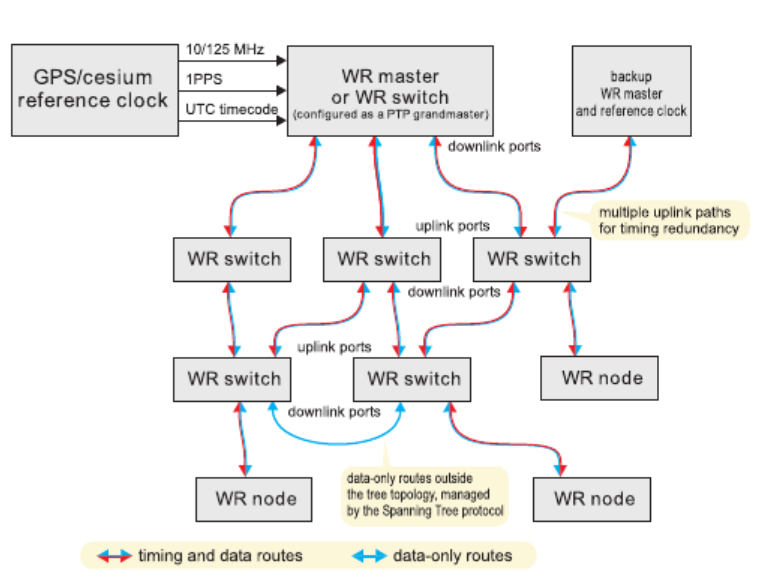
\includegraphics[width=0.7\linewidth]{imagenes/wr_topology}
	\caption[Topología de red en WR]{Gráfico de una topología de red típica en 
	WR. Imagen tomada de \cite{Daniluk2012}.}
	\label{fig:wrtopology}
\end{figure}

El sentido de las señales de temporización en la red es siempre descendente, es 
decir, cada equipo se sincroniza con el que está conectado directamente a él en 
un nivel superior y así hasta llegar a la raíz. También se puede dar el caso de 
que existan equipos que actúan a la manera de los TC de PTP y realizar la 
sincronización siguiendo un esquema \textit{peer-to-peer}, como se vio en la 
sección de PTP, aunque esto es algo que está actualmente desarrollándose, por 
lo que el esquema típico es \textit{end-to-end}. Se ha dicho con anterioridad 
que los equipos WR permiten el paso de tráfico general a través de ellos, 
permitiendo reutilizar la red de distribución de tiempo para el envío de 
tráfico estándar. En este caso no se restringe al esquema jerárquico: los 
paquetes pueden viajar a cualquier nodo de la red sin restricciones, es decir, 
como en una red Ethernet estándar.

\subsection{Modelo de enlace}

Uno de los aspectos que limitaban el rendimiento al protocolo PTP era la 
consideración de simetría entre los caminos de ida y vuelta de los paquetes por 
el enlace. En WR se hace una separación de ambos caminos de manera que se 
estima de forma bastante precisa el tiempo empleado en el sentido maestro a 
esclavo que posteriormente se utiliza para calcular el desfase. ¿Como se 
consigue dicha estimación? WR tiene como requisito el uso de enlaces de fibra 
óptica bidireccionales, lo que conlleva que físicamente la longitud del enlace 
es idéntica en ambos sentidos. Sin embargo, dado que se deben emplear dos 
longitudes de onda distintas para permitir una comunicación 
\textit{Full-Duplex} la realidad es que el tiempo de propagación no es 
simétrico lo que supone que no es igual transmitir en sentido maestro a esclavo 
que en el contrario. La solución que se aplica es la caracterización de dicha 
diferencia y la inclusión de un parámetro en el modelo que permite separar el 
tiempo de ida del \textit{round-trip} total. Para ello se sigue un proceso de 
calibración que relaciona las dos longitudes de onda empleadas en el enlace de 
comunicación siguiendo la expresión en \ref{eq:alpha}. La gran ventaja de este 
método es que se permite calibrar el 
enlace de forma dinámica. Dado que se posee la relación existente entre 
transmitir en una longitud de onda y recibir en otra, cogiendo el tiempo total 
y aplicando dicha relación a él se puede extraer el tiempo empleado en un 
sentido. Además es necesario caracterizar los retardos de la electrónica a fin 
de eliminar asimetrías entre los distintos dispositivos que pueden encontrarse 
en la red WR, el proceso de calibración completo se define en \cite{man:calib}.

\begin{equation}\label{eq:alpha}
\alpha = \frac {\delta_{MS} - \delta_{SM}} {\delta_{SM}}
\end{equation}

\subsection{Algoritmo}

El algoritmo de corrección de desfase para el reloj local se parece a los ya 
vistos anteriormente donde se realizaba una serie de intercambios de paquetes 
sellados mediante los que se realizaba el cálculo del tiempo de propagación y 
del desfase. WR añade complejidad a este proceso ya que inicialmente se debe 
realizar una fase de sintonización, a la que sigue la de seguimiento de fase 
del reloj maestro. De forma resumida se siguen los siguientes pasos:

\begin{enumerate}
	\item Inicialmente el maestro codifica su reloj de referencia y comienza a 
	mandar paquetes de presencia a la red.
	
	\item El nodo esclavo recibe los paquetes y recupera la señal de reloj de 
	referencia codificada que es una copia exacta del reloj del nodo maestro 
	con un desfase correspondiente al tiempo de transmisión de los paquetes 
	entre el nodo maestro y el esclavo ($delay_{MS}$).
	
	\item Se ajusta el reloj denominado \textit{helper} en el nodo esclavo y se 
	desfasa en un valor fijo conocido.
	
	\item Ahora el nodo esclavo (que ya posee el reloj \textit{helper} 
	sintonizado y desfasado con un valor fijo $phase_s$) realiza la misma 
	operación de ajuste de su reloj de referencia y lo emplea para la 
	codificación y envío de paquetes al nodo maestro. Una vez finalizado el 
	proceso este reloj de referencia sería una copia exacta del reloj del 
	maestro tanto en frecuencia como en fase.
	
	\item El maestro recupera dicho reloj y mide la diferencia de fase entre 
	este y su reloj de referencia. Este valor se denomina $phase_{MM}$ y se 
	expresa de la siguiente forma:
	\begin{equation}\label{eq:phasemm}
	phase_{MM} = (\Delta + \delta_{ms} + \delta_{sm} + phase_s) mod T_{ref}
	\end{equation}
	donde $\Delta$ es la suma de todos los retardos fijos en los circuitos de 
	transmisión y recepción así como valores de propagación en la electrónica 
	de la tarjeta, y $T_{ref}$ es el periodo del reloj físico usado para el 
	enlace Ethernet (para el caso de un enlace Gigabit sería 8 ns o 125 MHz).
\end{enumerate}

El diagrama mostrado en la Figura \ref{fig:wrsync} muestra de manera gráfica 
los pasos enumerados anteriormente en el proceso de sincronización para el 
protocolo WR. Este protocolo consigue reducir la resolución de las marcas de 
tiempo (teóricamente limitadas por un ciclo del reloj de enlace) empleando una 
serie de módulos denominados \gls{ddmtd} que permiten realizar mediciones de 
desfase con una exactitud de femtosegundos. Estas medidas se utilizan como 
entrada por un algoritmo de control PI que calcula los valores de consigna 
empleados en corregir el reloj local para que siga al reloj del maestro.

\begin{figure}
	\centering
	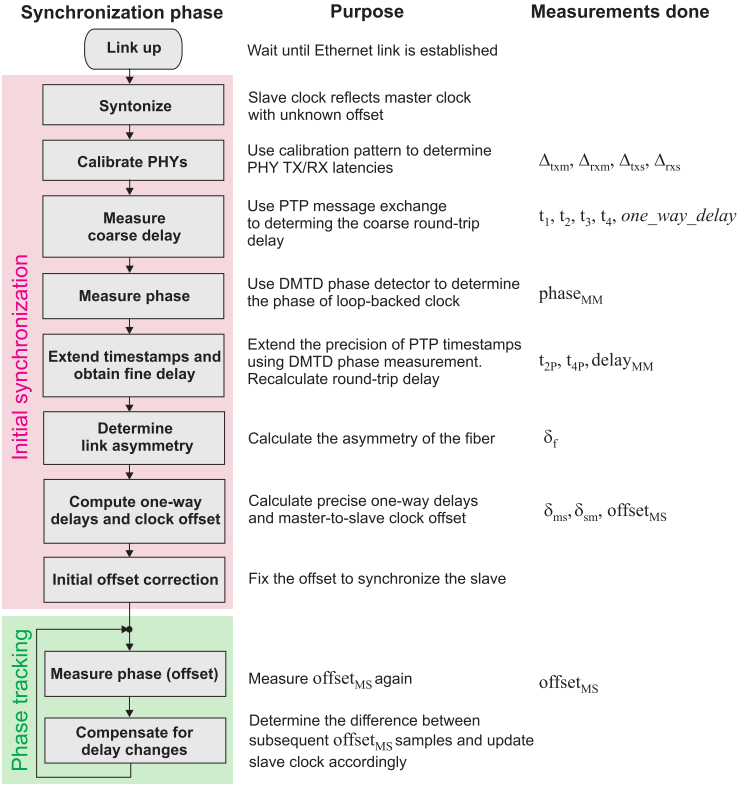
\includegraphics[width=\linewidth]{imagenes/wr_sync}
	\caption[Etapas del proceso de sincronización WR]{Etapas del proceso de 
	sincronización WR. Imagen tomada de \cite{Wlostowski2011}.}
	\label{fig:wrsync}
\end{figure}

\subsection{Arquitectura para nodos WR}

Los dispositivos que incorporan la tecnología WR presentan dos tipos de 
arquitecturas.

\begin{itemize}
	\item La arquitectura para \textit{switch} que se ilustra en la Figura 
	\ref{fig:switchhdl}. Se caracteriza por incluir un procesador físico tipo 
	ARM de manera externa a la FPGA. Este se comunica mediante accesos mapeados 
	a memoria con el resto de los componentes incluidos como módulos VHDL. El 
	elemento de interconexión es el bus Wishbone de tipo barras cruzadas, que 
	tiene la característica de permitir la coexistencia de varios maestros del 
	bus. El módulo \textit{RT subsystem} encapsula un segundo nivel de bus 
	donde se incluye un microprocesador embebido, el LM32 de Lattice, cuyo 
	propósito es ejecutar un \text{sw} con requisitos de tiempo real que se 
	encarga del cómputo del desfase entre el reloj recuperado del maestro y el 
	local.
	
	\begin{figure}
		\centering
		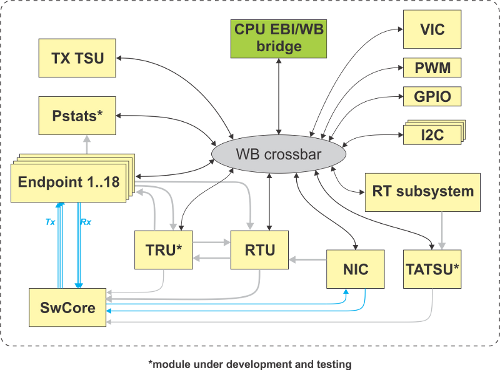
\includegraphics[width=\linewidth]{imagenes/switch_hdl}
		\caption[Diagrama de los componentes de la arquitectura del WRS]{Este 
		diagrama muestra la estructura interna de módulos que componen la 
		arquitectura del WRS. El elemento central es el bus Wishbone al que se 
		conectan el resto de periféricos. El procesador puede acceder a dichos 
		periféricos mdiante accesos mapeados a memoria.}
		\label{fig:switchhdl}
	\end{figure}
	
	\item La arquitectura para \textit{nodo} correspondiente a la Figura 
	\ref{fig:wrpcinside}. En este caso vemos como se ha prescindido de varios 
	delos módulos presentes en la arquitectura de \textit{switch} de manera que 
	queda un diseño más sencillo pensado para FPGAs de perfil bajo. No hay 
	soporte de un microprocesador externo por lo que toda la lógica encargada 
	de la gestión del protocolo, de las herramientas de gestión y demás debe 
	ser implementada como \textit{sw} embebido en el LM32. El número de 
	interfaces físicas se reduce a 1 de manera que los dispositivos que 
	incorporen esta arquitectura solo pueden operar como OC.
\end{itemize}

\begin{figure}
	\centering
	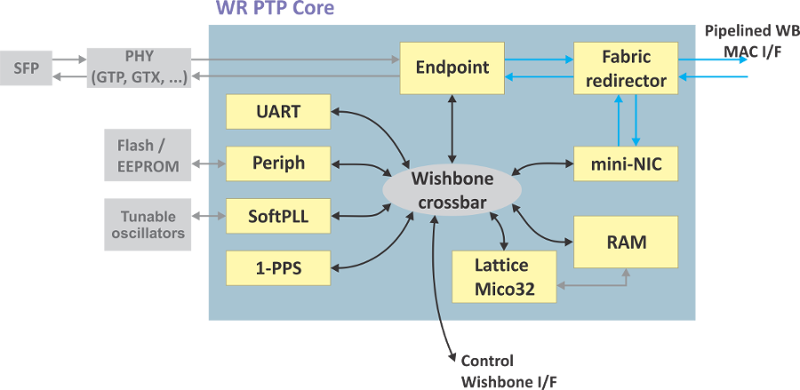
\includegraphics[width=\linewidth]{imagenes/wrpc_inside}
	\caption[Esquema de bloques del WR PTP Core]{En este esquema de bloques se 
		incluyen los componentes principales que componen la arquitectura del 
		WR 
		PTP Core. El bloque principal hace referencia a los componentes en la 
		parte 
		de lógica repogramable, mientras que fuera se incluyen componentes que 
		o 
		bien se incluyen como soporte hw dentro de la FPGA (PHY) o bien son 
		componentes externos que se conectana a algún pin para comunicarse con 
		los 
		elementos internos. Imagen tomada de \cite{Daniluk2012}.}
	\label{fig:wrpcinside}
\end{figure}

Ambas arquitecturas son plenamente funcionales y se encuentran incluidas en los 
dispositivos de referencia como el WRS (para rol de BC) y la tarjeta SPEC 
\cite{website:specwiki} (OC). 

\subsection{Rendimiento}

El protocolo WR permite sincronizar un gran número de nodos con una exactitud 
inferior al nanosegundo. Esto es algo ya de por si relevante pero que a fin de 
cuentas es un tema de calibración de los retardos ocasionados por los 
componentes que intervienen en el enlace. El verdadero punto fuerte es la 
precisión que alcanza en el orden de los picosegundos y que confiere una gran 
ventaja con respecto a protocolos como PTP o NTP donde la precisión se 
encuentra en varios órdenes de magnitud por encima. Mejorar la exactitud pasa 
directamente por reducir las perturbaciones que afectan al sistema y que 
repercuten en la precisión de las señales generadas. Los valores numéricos en 
cuanto al rendimiento de la sincronización en WR se pueden encontrar en los 
capítulos 4 y 6.